\documentclass[aps,prb,superscriptaddress,nofootinbib]{revtex4}
\usepackage{amsfonts}
\usepackage{amsmath}
\usepackage{amssymb}
\usepackage{graphbox}
\usepackage{graphicx}
\usepackage{caption}
\usepackage{bm}
\usepackage{bbm}
\usepackage{cancel}
\usepackage{color}
\usepackage{mathrsfs}
\usepackage[colorlinks,bookmarks=true,citecolor=blue,linkcolor=red,urlcolor=blue]{hyperref}
\usepackage{simpler-wick}
\usepackage{appendix}
\usepackage{float}
\usepackage{array}
\usepackage{booktabs}
\usepackage[export]{adjustbox}
\setlength{\parindent}{10 pt}
\setlength{\parskip}{2 pt}
\setcounter{MaxMatrixCols}{30}
\bibliographystyle{apsrev}
\newcommand{\RNum}[1]{\uppercase\expandafter{\romannumeral #1\relax}}
\newcommand{\normord}[1]{{:\mathrel{#1}:}}
\def\tbs{\textbackslash}
\def \tr{\operatorname{tr}}
\def \Tr{\operatorname{Tr}}


\begin{document}
\title{Fermi Liquid}
\author{Jie Ren}



\maketitle

\tableofcontents


\section{RG for 1D Fermi Liquid}

In this section, we gives a field theoretical analysis of the interacting fermion system in 1D.
For the notational simplicity, we shift the momentum so that
\begin{equation}
	k \rightarrow k' = \begin{cases}
		k - k_F & r=R \\
		-k - k_F & r=L
	\end{cases}.
\end{equation}
The dispersion is then $\varepsilon_r(k) = v_F k$.
In this way, two Fermi points are brought to the origin, the left and right moving branches have the same dispersion.
The integral over momentum shell for both species of fermion can then be denoted by
\begin{equation}
	\int^\Lambda \frac{dK}{2\pi} \equiv \int_{-\Lambda}^\Lambda \frac{dk_L}{2\pi} + \int_{-\Lambda}^\Lambda \frac{dk_R}{2\pi}.
\end{equation}



\subsection{Effective Field Theory}

The effective field theory for the free field is
\begin{equation}
	Z_0 = \prod_{r=L/R}\int D\left[\bar\psi_r(k,\omega),\psi_r(k,\omega)\right] e^{-S_0},
\end{equation}
where the free field action is
\begin{equation}
	S_0 = \sum_{r=L/R} \int^\Lambda_{-\Lambda} \frac{dk}{2\pi} \int^\infty_{-\infty} \frac{d\omega}{2\pi} 
	\bar\psi_r(k,\omega)[-i\omega + v_F k]\psi_r(k,\omega),
\end{equation}
which gives the free field propagator:
\begin{equation}
	G_r(k,\omega) = -\langle \psi_r(k,\omega)\bar\psi_r(k,\omega)\rangle�
	= \frac{1}{i\omega - v_F k}.
\end{equation}
We then consider the rescaling of the cut-off $\Lambda \rightarrow \Lambda/s$. 
To make the free action scale invariant, we define the rescaled variables:
\begin{equation}
	k' = sk, \quad \omega' = s\omega, \quad 
	\psi'_r(k',\omega') = s^{-3/2}\psi_r(k,\omega).
\end{equation}
Then we consider the perturbation from quadratic and quartic terms:
\begin{equation}
\begin{aligned}
	\delta S_2 &= \sum_{r=L/R} \int^\Lambda_{-\Lambda}\frac{dk}{2\pi}\int^\infty_{-\infty} \frac{d\omega}{2\pi} 
	\mu(k,\omega) \bar\psi_r(k,\omega) \psi_r(k,\omega), \\
	\delta S_4 &= \frac{1}{2!2!} \int^\Lambda_{K,\omega} 
	u(4,3,2,1)\bar\psi(4)\bar\psi(3)\psi(2)\psi(1),
\end{aligned}
\end{equation}
where we have suppressed the momentum labels: 
\begin{equation}
	\psi(i) = \psi_{r_i}(k_i,\omega_i), \quad
	u(4,3,2,1) = u(K_4,\omega_4;K_3,\omega_3;K_2,\omega_2;K_1,\omega_1),
\end{equation}
and the integral is defined as:\footnote{The symbol $\bar\delta$ enforces momentum conservation mod $2\pi$, as is appropriate to any lattice problem. A process where lattice momentum is violated in multiples of $2\pi$ is called an \textit{umklapp process}.}
\begin{equation}
\begin{aligned}
	\int_{K \omega}^{\Lambda}
	=& \ \int^\Lambda \frac{d K_1 \cdots d K_4}{(2 \pi)^{4}} \int_{-\infty}^{\infty} \frac{d \omega_{1} \cdots d \omega_{4}}{(2 \pi)^{4}} \times 2 \pi \delta\left(\omega_{1}+\omega_{2}-\omega_{3}-\omega_{4}\right) \\
	&\ \times 2 \pi \bar{\delta}(K_1+K_2-K_3-K_4).
\end{aligned}
\end{equation}
Since this action separates into slow and fast pieces, the effect of mode elimination is simply to reduce $\Lambda$ to $\Lambda/s$ in the integral above. Rescaling moments and fields, we find that
\begin{equation}
	\mu'(k',\omega') = s\cdot\mu\left(\frac{k'}{s}, \frac{\omega}{s}\right).
\end{equation}
Expand $\mu$ in series:
\begin{equation}
	\mu(k, \omega)=\mu_{00}+\mu_{10} k+\mu_{01} i \omega+\cdots+\mu_{n m} k^{n}(i \omega)^{m}+\cdots,
\end{equation}
and compare both sides. The constant piece is a relevant perturbation.
This relevant flow reflects the readjustment of the Fermi sea to a change in chemical potential. 
The correct way to deal with this term is to include it in the free-field action by filling the Fermi sea to a point that takes $\mu_{00}$ into account. 
The next two terms are marginal and modify terms that are already present in the action.

We now turn on the quartic interaction, the dimensional analysis gives the transformation of $u$:
\begin{equation}
	u'_{i_4,i_3,i_2,i_1}(k'_i,\omega'_i) = u_{i_4,i_3,i_2,i_1}\left(\frac{k'_i}{s},\frac{\omega'_i}{s}\right).
\end{equation}
If we expand $u$ in a Taylor series in its arguments and compare coefficients, we find that the constant term u0 is marginal and the higher coefficients are irrelevant. 
Thus, $u$ depends only on its discrete labels and we can limit the problem to just a few coupling constants instead of the coupling function we started with. 
Furthermore, all reduce to just one coupling constant:
\begin{equation}
	u_0 = u_{LRLR} = u_{RLRL} = -u_{RLLR} = -u_{LRRL} \equiv u.
\end{equation}
Other couplings corresponding to the ($LL \rightarrow RR$) process are wiped out by the Pauli principle since they have no momentum dependence and cannot have the desired antisymmetry.

\subsection{RG at One-loop Level}

Consider the infinitesimal rescale $s=e^{dt}$. 
The one-loop contribution to the quadratic term is\footnote{We include an infinitesimal $e^{i\omega\eta}$ to ensure convergence as we do the integral over $\omega$ by closing the upper half-plane.}
\begin{equation}
	\mu^{(2)}_{LL} = 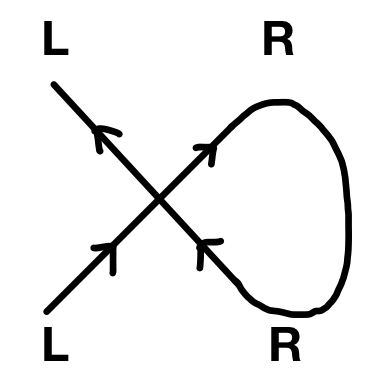
\includegraphics[align=c, width=0.125\linewidth]{pics/FL-1.png}
	= -u \int_{d\Lambda} \frac{dk}{2\pi}\int^\infty_{-\infty}\frac{d\omega}{2\pi}\frac{e^{i\omega \eta}}{i\omega - v_F k},
\end{equation}
where the integral on the momentum shell is
\begin{equation}
	\int_{d\Lambda}\frac{dk}{2\pi} = \int_{-\Lambda}^{-\Lambda(1-dt)} \frac{dk}{2\pi} + \int_{\Lambda(1-dt)}^{\Lambda} \frac{dk}{2\pi}.
\end{equation}
The result gives:
\begin{equation*}
	\mu^{(2)}_{LL}
	= -\frac{u\Lambda}{2 \pi}dt.
\end{equation*}
By the symmetry $L \leftrightarrow R$, we know $\mu^{(2)}_{LL}=\mu^{(2)}_{RR}=\mu^{(2)}$, so the RG flow is
\begin{equation}
	\frac{d}{dt}\left[s\cdot\left(\mu+\mu^{(2)}\right)\right] = \mu - \frac{u\Lambda}{2\pi}.
\end{equation}
The one-loop correction to the quartic term ($u_{LRRL}=-u$) have two contributions.
One is called ZS' (zero sound) channel:\footnote{There is actually another zero sound channel ZS, but which has no contribution to the vertex because the diagram contains the vertex of the ($LL \rightarrow RR$) process, which has no relevant contribution the the vertex.}
\begin{equation}
\begin{aligned}
	u^{(2)}_{\mathrm{ZS'}} 
	&= 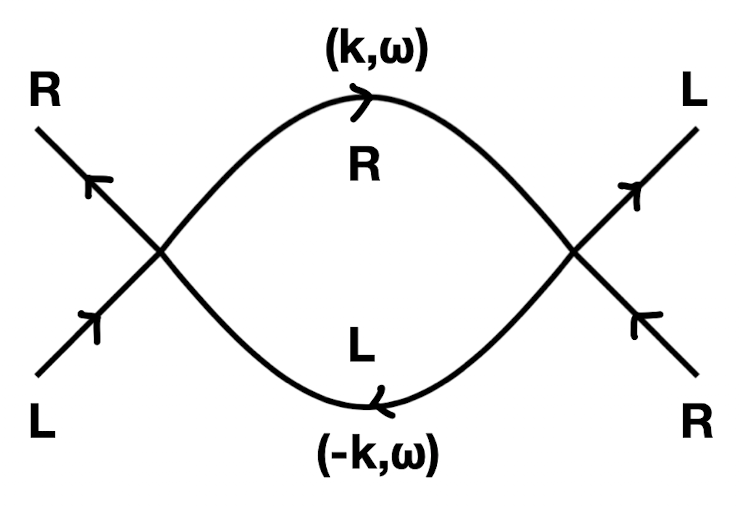
\includegraphics[align=c, width=0.2\linewidth]{pics/FL-2.png} \\
	&= -u^2 \int^\infty_{-\infty}\int_{\Lambda/s<|k|<\Lambda} \frac{d\omega dk}{(2\pi)^2} \frac{e^{i\omega\eta}}{(i\omega+v_F k)(i\omega-v_F k)} \\
	&= u^2\int_{\Lambda/s<|k|<\Lambda} \frac{dk}{2\pi} \frac{1}{2|k|} \\
	&= \frac{u^2}{2\pi}\frac{d\Lambda}{\Lambda}.
\end{aligned}
\end{equation}
The sign is obtained from contracting the Fermion field monomial:
\begin{equation*}
	\wick{
        \c1 {\bar\psi}_L \bar\psi_R \psi_L \c2 \psi_R
        \bar\psi_L \c2 {\bar\psi}_R \c1 {\psi}_L \psi_R
	} = -G_L G_R \bar\psi_R \psi_L \bar\psi_L \psi_R
	= -G_L G_R \bar\psi_L \bar\psi_R \psi_L \psi_R.
\end{equation*}
The other is called the BCS channel:\footnote{The $1/2$ factor comes from the symmetry factor of the diagram.}
\begin{equation}
	u^{(2)}_{\mathrm{BCS}} 
	= 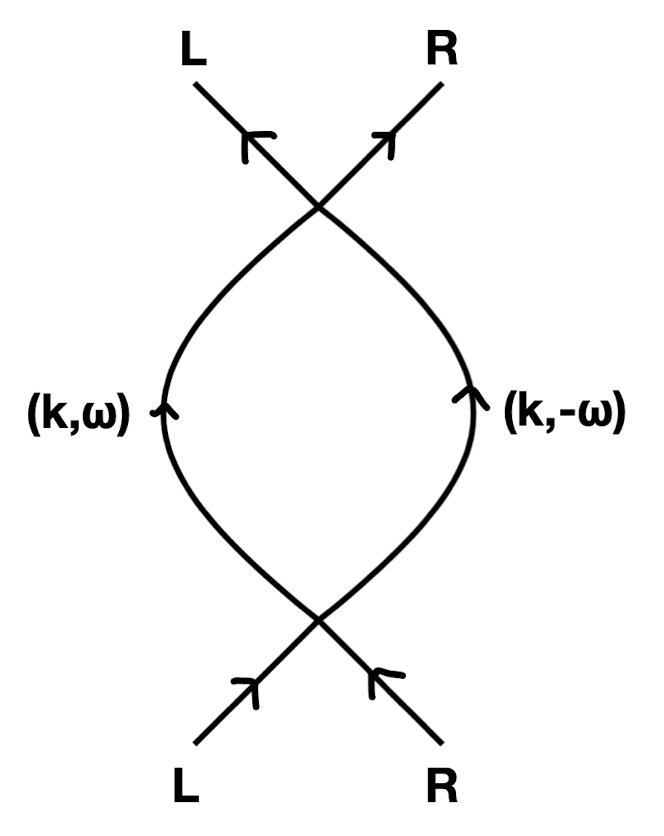
\includegraphics[align=c, width=0.15\linewidth]{pics/FL-3.png} 
	= -\frac{u^2}{2} \sum_{r=L/R}\int^\infty_{-\infty}\int_{d\Lambda} \frac{d\omega dk_i}{(2\pi)^2} \frac{e^{i\omega\eta}}{(i\omega-v_F k)(-i\omega-v_F k)}.
\end{equation}
The sign is obtained from the contraction:
\begin{equation*}
	\wick{
        \bar\psi_L \bar\psi_R \c1 \psi_L \c2 \psi_R
        \c1 {\bar\psi}_L \c2 {\bar\psi}_R \psi_L \psi_R
	} = -G_L G_R \bar\psi_L \bar\psi_R \psi_L \psi_R.
\end{equation*}
Note that we will obtained a factor of 2 since in this channel, the intermedia propagator can be left mover or right mover.
We see that two contributions cancel out:
\begin{equation}
	u^{(2)}_{\mathrm{ZS'}} + u^{(2)}_{\mathrm{BCS}} = 0.
\end{equation}
Together, the RG flow to the one-loop level is
\begin{equation}
	\frac{d\mu}{dt} = \mu - \frac{u\Lambda}{2\pi}, \quad
	\frac{du}{dt} = 0.
\end{equation}
The fixed point solution to the RG flow is:
\begin{equation}
	\mu^* = \frac{u^*\Lambda}{2\pi},
\end{equation}
where the fixed-point value of $u^*$ is arbitrary. 
The vanishing beta function predict that at least for small interaction, the system does not immediately develop a CDW order.
However, as the vertex function is marginal in the RG analysis, the fix points become a fixed line.
When the coupling $u$ is nonzero, the analysis for the Gaussian fix point becomes untrustworthy.
Actually when $u$ is getting sufficiently large, the umklapp process becomes relevant and the system flows to CDW phase.
A more systematic analysis requires the bosonization techniques. 



\section{RG of 2D Fermi Liquid}
In this section, we are considering the system of weakly interacting Fermi gas.
To be specific, we consider the lattice Hamiltonian:
\begin{equation}\label{eq:FL-gen-ham}
	H = -\frac{1}{2}\sum_{\langle i,j \rangle} (c_i^\dagger c_{j} + c_{j}^\dagger c_i) + \mu\sum_i c_i^\dagger c_i + \sum_{i,j,k,l} u_{ijkl} c_i^\dagger c_j^\dagger c_k c_l.
\end{equation}
In the following, we investigate the effective field theory near the Fermi surface.
We discuss the RG flow of the couplings (mainly for two dimensional system).
Then we carry out the perturbative calculation for the correlation functions. 

\subsection{Effective Field Theory for Interacting Fermi Systems}
The low-energy manifold is an annulus of thickness $2 \Lambda$ symmetrically situated with respect to the Fermi circle $K=K_{\mathrm{F}}$.
The dispersion for the free lattice model is
\begin{equation}
	E(\bm K) = -\cos K_x - \cos K_y \simeq -2 + \frac{\bm K^2}{2}.
\end{equation}
For a given chemical potential $\mu$, the Fermi circle is $K_F = \sqrt{2m\mu}$, we can linearize the dispersion near the Fermi surface:
\begin{equation}
	E(\bm K) = \frac{\bm K^2-K_F^2}{2m} \simeq \frac{K_F}{m}k \equiv v_F k, \quad
	k\equiv |K|-K_F
\end{equation}
The partition function is:
\begin{equation}
	Z_0 = \sum_\theta \sum_{|k|<\Lambda}\int D\left[\bar\psi(k,\theta,\omega),\psi(k,\theta,\omega)\right] e^{-S_0},
\end{equation}
where the free field action is:\footnote{A factor of $K_{\mathrm{F}}$ has been absorbed in the field.}
\begin{equation}
	S_0 = \int \frac{d\theta}{2\pi} \int^\Lambda_{-\Lambda}\frac{dk}{2\pi} \int^\infty_{-\infty}\frac{d\omega}{2\pi} \bar\psi(k,\theta,\omega)(-i\omega+v_F k)\psi(k,\theta,\omega).
\end{equation}
Consider the quartic interaction
\begin{equation}
	\delta S_4 = \frac{1}{4}\int_{\bm K,\theta,\omega} \bar\psi(4)\bar\psi(3)\psi(2)\psi(1)u(4,3,2,1)
\end{equation}
where we eliminate one of the four sets of variables, say, the one numbered 4, by integrating them against the delta functions:
\begin{equation}
	\int_{K,\theta,\omega}
	=\prod_{i=1}^{3} \int_{0}^{2 \pi} \frac{d \theta_{i}}{2 \pi} \int_{-\Lambda}^{\Lambda} \frac{d k_{i}}{2 \pi} \int_{-\infty}^{\infty} \frac{d \omega_{i}}{2 \pi} \theta\left(\Lambda-\left|k_{4}\right|\right), \quad 
	k_4 = |\bm K_4|-K_F.
\end{equation}
The $\omega$ integral is easy: since all $\omega$'s are allowed, the condition $\omega_4=\omega_1+\omega_2-\omega_3$ is always satisfied for any choice of the first three frequencies. 
The same would be true for the momenta if all momenta were allowed. 
But they are not; they are required to lie within the annulus of thickness $2\Lambda$ around the Fermi circle. 
Consequently, if one freely chooses the first three momenta from the annulus, the fourth could have a length as large as $3K_F$. 
The role of $\delta(\Lambda-|k_4|)$ is to prevent exactly this.

\subsubsection*{Momentum Constraint}
Note that $k_4$ can be expressed as
\begin{equation}
	k_4 = |(K_F+k_1)\bm \Omega_1+(K_f+k_2)\bm \Omega_2-(K_F+k_3)\bm \Omega_3|-K_F.
\end{equation}
When doing RG towards the Fermi surface, the integral measure will not preserve the preserve the original form.
The situation is clearly is we use a smooth cutoff
\begin{equation}
	\theta(\Lambda-|k_4|) \rightarrow e^{-|k_4|/\Lambda},
\end{equation}
and define $\Delta\equiv \bm \Omega_1+\bm \Omega_2-\bm \Omega_3$, $k_4$ in this way behaves as
\begin{equation}
	k_4 = (|\Delta|-1)K_F + O(k).
\end{equation}
The integral then change to:
\begin{equation}
\begin{aligned}
	& \prod_{i=1}^{3} \int_{-\Lambda}^{\Lambda} \frac{d k_{i}}{2\pi} 
		\int \frac{d \theta_{i}}{2 \pi} \int \frac{d \omega_{i}}{2 \pi} 
		e^{-||\Delta|-1|\frac{K_F}{\Lambda}} u(k,\theta,\omega) 
		\bar\psi \bar\psi \psi \psi \\
	\overset{\mathrm{RG}}{\longrightarrow} & \prod_{1}^{3} \int_{-\Lambda}^{\Lambda}
		\frac{d k_{i}^{\prime}}{2 \pi} 
		\int \frac{d \theta_{i}}{2 \pi} 
		\int \frac{d \omega_{i}^{\prime}}{2 \pi} 
		e^{-|| \Delta|-1|\frac{sK_F}{\Lambda}} 
		u\left(\frac{k^{\prime}}{s} \frac{\omega^{\prime}}{s} \theta\right) 
		\bar\psi \bar\psi \psi \psi.
\end{aligned}
\end{equation}
We can then get the RG transformation of $u$ as
\begin{equation}
	u'(k',\theta,\omega') = e^{-||\Delta|-1|\frac{(s-1)K_F}{\Lambda}}u\left(\frac{k'}{s},\theta,\frac{\omega'}{s}\right).
\end{equation}
By Taylor expansion, we conclude that the only couplings that survive the RG transformation without any decay correspond to the cases in which $|\Delta|=1$, and without momentum dependence.

\begin{figure}[]
	\centering
	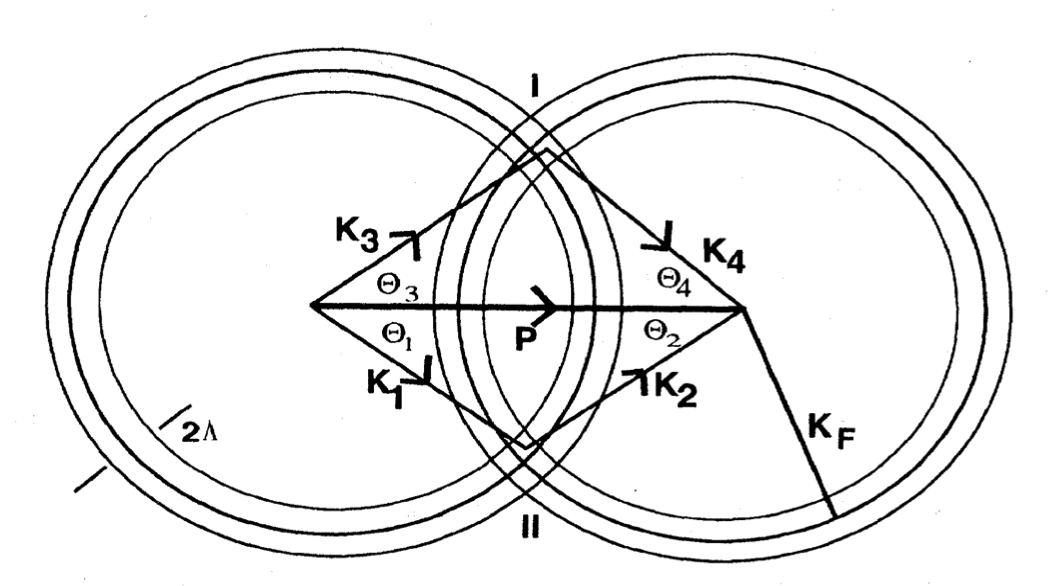
\includegraphics[hsmash=c,width=0.4\linewidth]{pics/FL-kcons.png}
	\caption{The geometric construction for determining the allowed values of momenta. If $K_{1}$ and $K_{2}$ add up to $P$, then $K_{3}$ and $K_{4}$ are constrained as shown, if they are to add up to $P$ and lie within the cutoff. If the incoming momenta $K_{1}$ and $K_{2}$ are equal and opposite, the two shells coalesce and $K_{3}$ and $K_{4}$ are free to point in all directions, as long as they are equal and opposite.}
	\label{fig:FL-kcons}
\end{figure}

This equation has only three solutions (see also Fig.~\ref{fig:FL-kcons}):
\begin{equation}
\begin{aligned}
	&\text{Case I:} \quad \bm \Omega_1 = \bm \Omega_3, \\
	&\text{Case II:} \quad \bm \Omega_2 = \bm \Omega_3, \\
	&\text{Case III:} \quad \bm \Omega_1 = -\bm \Omega_2.
\end{aligned}
\end{equation}
Because of the rotational symmetry, the marginal vertex functions are determined solely by two functions:
\begin{eqnarray}
	u[\theta_1,\theta_2,\theta_1,\theta_2] &\equiv& F(\theta_1,\theta_2) = F(\theta_1-\theta_2), \\
	u[\theta_1,\theta_2,\theta_2,\theta_1] &=& -F(\theta_1-\theta_2), \\
	u[\theta_1,-\theta_1,\theta_3,-\theta_3] &\equiv& V(\theta_1,\theta_3) = V(\theta_1-\theta_3).
\end{eqnarray}
Note that the manifestation of the Pauli principle on $F$ and $V$ is somewhat subtle: $F$ will not be antisymmetric under $1 \leftrightarrow 2$ since, according to the way it is defined above, we cannot exchange 1 and 2 without exchanging 3 and 4 at the same time. 
On the other hand, since 3 and 4 can be exchanged without touching 1 and 2 in the definition of $V$, $V$ must go to $-V$ when $1 \leftrightarrow 3$.

\subsection{One-loop RG for 2D System}
We first consider the loop correction to the chemical potential:
\begin{equation}
\begin{aligned}
	\mu^{(2)}(k,\theta,\omega) 
	&= \int_{d\Lambda}\frac{dK'}{2\pi} \int \frac{d\omega'}{2\pi} \int \frac{d\theta'}{2\pi} \frac{F(\theta-\theta')}{i\omega-v_F k'} \\
	&= \int_{-\Lambda}^{-\Lambda+\Lambda dt}\frac{dK'}{2\pi} \int \frac{d\theta'}{2\pi} F(\theta-\theta') \\
	&= \frac{\Lambda}{2\pi} \left[\int\frac{d\phi}{2\pi} F(\phi)\right] dt.
\end{aligned}
\end{equation}
For the vertex correction, again we should consider three channels corresponding to the diagrams:
\begin{equation}
	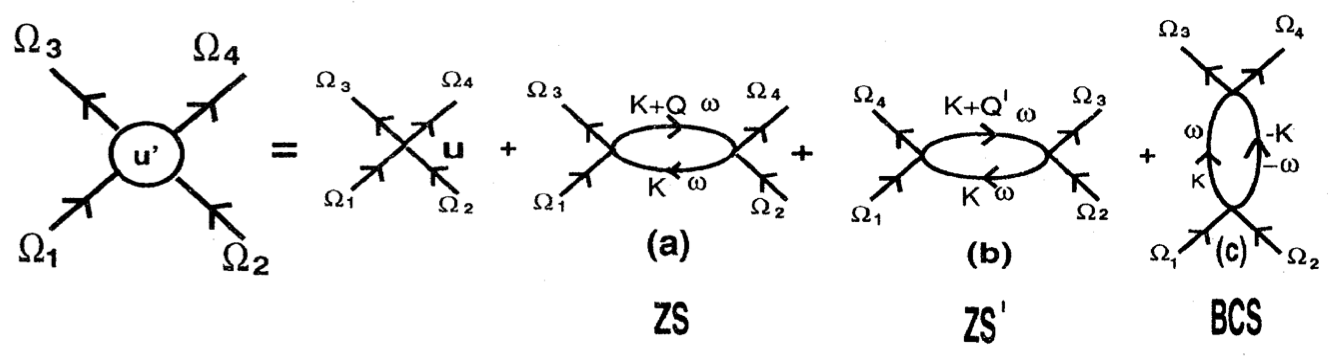
\includegraphics[align=c, width=0.7\linewidth]{pics/FL-4.png}
\end{equation}
First we consider the correction to the $F(\theta)$.
The contribution from the ZS channel (the momentum transfer $Q \simeq 0$) is
\begin{equation}
	F^{(2)}_{\mathrm{ZS}}(\theta_1-\theta_2) = \int_{d\Lambda}\frac{dk}{2\pi}\int \frac{d\omega}{2\pi} \int \frac{d\theta}{2\pi} \frac{F(\theta_1-\theta)F(\theta-\theta_2)}{(i\omega-v_F k)^2}.
\end{equation}
Since two poles of the integrant lie at the same half plane, we can alway choose to close the loop integral along the other half, and thus getting zero contribution.

\begin{figure}[]
	\centering
	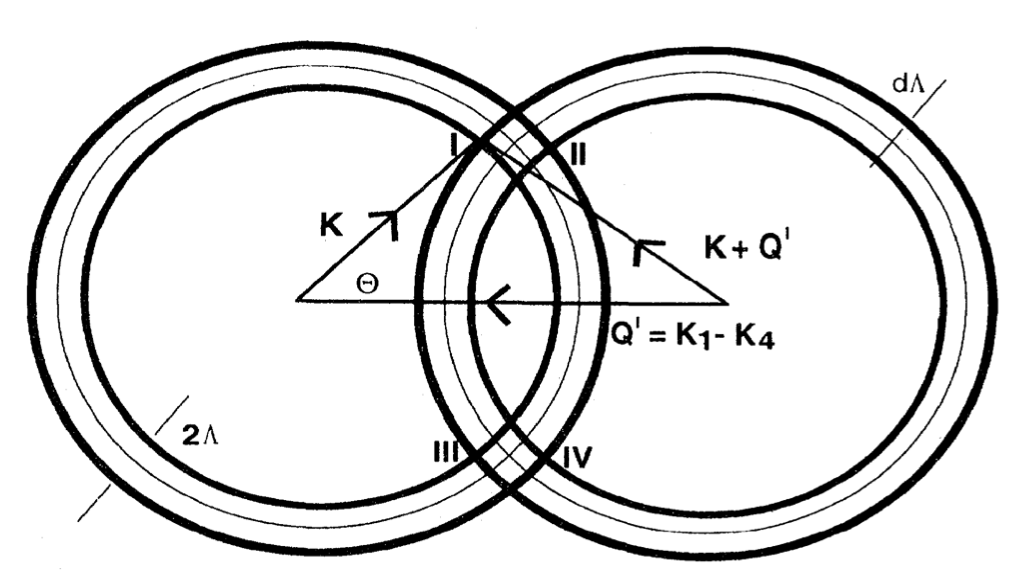
\includegraphics[hsmash=c,width=0.4\linewidth]{pics/FL-kshell.png}
	\caption{Construction for determining the allowed values of loop momenta in ZS'. The requirement that the loop momenta come from the shell and differ by $Q'$ forces them to lie in one of the eight intersection regions of width $d\Lambda^2$.}
	\label{fig:FL-kshell}
\end{figure}

For the ZS' channels, the momentum conservation condition (see Fig.~\ref{fig:FL-kshell}) restrict the phase space to be of order $d\Lambda^2$, and thus has no relevant contribution to $F(\theta)$.
Finally, for the same kinematical reason, the BCS diagram does not renormalize $F(\theta)$ at one loop.
Consider Fig.~\ref{fig:FL-kcons}, with $K_3$ and $K_4$ replaced by the two momenta in the BCS loop, $K$ and $P-K$.
In each annulus we keep just two shells of thickness $d\Lambda$ at the cutoff corresponding to the modes to be eliminated. 
The requirement that $K$ and $P-K$ lie in these shells and also add up to $P$ forces them into intersection regions of order $d\Lambda^2$. 
This means the diagram is just as ineffective as the ZS' diagram in causing a flow. 
Thus any $F$ is a fixed point to this order.

Now we consider the correction to the $V(\theta)$ function.
We choose the external momenta equal and opposite and on the Fermi surface. 
The ZS and ZS' diagrams do not contribute to any marginal flow for the same reason that BCS and ZS' did not contribute to the flow of $F(\theta)$.
But the BCS diagram produces a flow:
\begin{equation}
\begin{aligned}
	V^{(2)}_{\mathrm{BCS}}(\theta_1-\theta_3) 
	&= -\frac{1}{2}\int_{d\Lambda}\frac{dk}{2\pi}\int\frac{d\omega}{2\pi}\int\frac{d\theta}{2\pi} 
		\frac{V(\theta_1-\theta)V(\theta-\theta_3)}{(i\omega-v_F k)(-i\omega-v_F k)} \\
	&= -\frac{dt}{4\pi v_F}\int \frac{d\theta}{2\pi}V(\theta_1-\theta)V(\theta-\theta_3).
\end{aligned}
\end{equation} 
We can simplify the picture by going to angular momentum eigenfunctions,
\begin{equation}
	V(\theta) = \sum_l e^{il\theta} V_l,
\end{equation}
which gives the RG flow as
\begin{equation}
	\frac{dV_l}{dt} = -\frac{V_l^2}{4\pi v_F}.
\end{equation}
The solution to the RG flow is:
\begin{equation}
	V_l(t) = \frac{V_l(0)}{1+\frac{V_l(0)}{4\pi v_F}t}.
\end{equation}
What these equations tell us is that if the potential in angular momentum channel $l$ is repulsive, it will get renormalized (logarithmically) down to zero, while if it is attractive, it will run off to large negative values signaling the BCS instability. 
This is the reason the $V$'s are excluded in Landau theory, which assumes we have no phase transitions.\footnote{Remember that the sign of any given $V_l$ is not necessarily equal to that of the microscopic interaction. Kohn and Luttinger have shown (PRL, 15, 524 (1965)) that some of them will be always negative. Thus, the BCS instability is inevitable, though possibly at absurdly low temperatures or absurdly high angular momentum $l$.}




\end{document}


